\documentclass{article}

\usepackage{tikz}

\newlength{\size}

\newcommand{\gogrid}[1][1]{
  \setlength{\size}{\dimexpr#1cm/19\relax}

  \draw[step=\size] (-#1, -#1) grid (#1,#1);
  \draw[red,line width=1] (-#1, #1) -- (\dimexpr#1cm+1cm, #1);  % chktex 8
  \draw[blue,line width=1] (#1, -#1) -- (#1, #1);  % chktex 8
}

\begin{document}
  \begin{figure}[ht]
    \begin{center}
      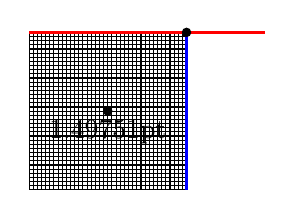
\begin{tikzpicture}
        \gogrid
        \filldraw (0,0) circle [radius=1.49751pt] node[below] {\the\size};
        \filldraw (1,1) circle[radius=1.49751pt];
      \end{tikzpicture}
      \caption{A grid with two points!}\label{my_grid1}
    \end{center}
  \end{figure}

  \begin{figure}[ht]
    \begin{center}
      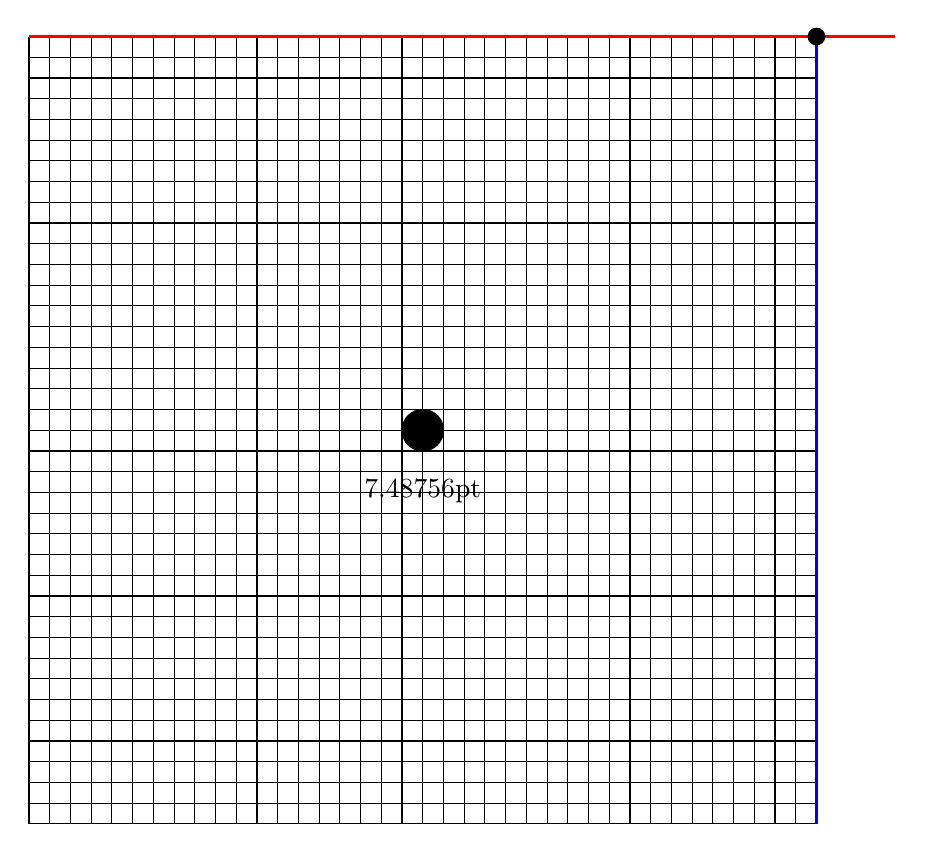
\begin{tikzpicture}
        \gogrid[5]
        \filldraw (0,0) circle [radius=7.48756pt] node[below=0.5cm] {\the\size};
        \filldraw (5,5) circle[radius=3pt];
      \end{tikzpicture}
      \caption{Another grid with two points!}\label{my_grid2}
    \end{center}
  \end{figure}
\end{document}